\documentclass[a4paper, 11pt]{scrartcl}
\usepackage[utf8]{inputenc}
\usepackage[ngerman]{babel}
\renewcommand{\familydefault}{\sfdefault}
\usepackage[a4paper]{geometry}
\usepackage{hyperref}
\usepackage{graphicx}
\usepackage[usenames,dvipsnames,svgnames]{xcolor}
\usepackage{amsmath}
\usepackage{lipsum}
\usepackage{verbatim}
\usepackage{listings}
\usepackage{soul}
\usepackage{titlesec}
\usepackage{booktabs}
\usepackage{tabu}
\usepackage{multirow}
\usepackage{graphicx}
\usepackage{enumitem}
\usepackage[justification=centering]{caption}

% Serifenfont für Überschriften
\setkomafont{disposition}{\normalcolor\bfseries}
% Seitengröße mit Geometry-Paket einstellen
\geometry{left=2.75cm,right=2.75cm,top=20mm,bottom=22mm,head=14.5pt}

\sethlcolor{lightgray}
\newcommand{\inlinecode}[1]{\hl{\texttt{#1}}}
\newcommand{\todo}[1]{\textbf{\color{red}{#1}}\normalcolor}

\title{Datenbankpraktikum -- Gruppe 3\\ Abschlusspräsentation}
\author{Janis Hamme, Karoly Kemeny, Thomas Neureuther,\\ Ming Niu, Alex Rubinshteyn,  Xinxin Yang}

\lstset{
    frame=top,frame=bottom,
    breaklines=true,
    captionpos=t,
    inputencoding={utf8},
    columns=fullflexible,
    breaklines=true
}

\lstset{literate=%
{Ö}{{\"O}}1
{Ä}{{\"A}}1
{Ü}{{\"U}}1
{ß}{{\ss}}2
{ü}{{\"u}}1
{ä}{{\"a}}1
{ö}{{\"o}}1
}


\titlelabel{\thetitle. }

\usepackage{parskip}
\setlength{\parindent}{0pt}
\setlength{\parskip}{0.5em}
\setlength{\belowcaptionskip}{-0.5em} 
\setlist[itemize]{itemsep=-0.25em}

\begin{document}

\maketitle

\section{Abbildung Semantischer Relationen (Aufgabe 3.2)}

\textbf{These}: \emph{''Bei Anfragen nach Adjektiven werden viele Synonyme, aber nur wenige Antonyme gefunden."}

Analyse von 100 Anfragen nach den 100 ähnlichsten Wörtern für zufällig gewählte Adjektive mit WordNet. Verwendet wurde der Amazon Produkt Datensatz mit 200er-Vektoren. Einmal unpartitioniert und unterteilt in 16 Partitionen.

\begin{table}[h!]
\centering
\begin{tabu}{lll}
\toprule
& \textbf{Unpartitioniert} & \textbf{Partitioniert} \\
\midrule
\textbf{Adjektive}&48.21\%&44.78\% \\
\textbf{Not Found}&21.84\%&24.59\%\\
\midrule
\textbf{Synonyme}&1.15\%&0.43\% \\
\textbf{Antonyme}&0.20\%&0.11\% \\
\textbf{keine Relation}&98.65\%&99.57\% \\
\bottomrule
\end{tabu}
\caption{Analyse mit Wordnet.}
\label{tbl:asdf}
\end{table}
Die Analyse (Tabelle 1) bestätigt zwar, dass sehr wenig Antonyme gefunden wurden, allerdings ist auch die Anzahl der Synonyme unter den Adjektiven erstaunlich klein. Die Partitionierung in 16 Partitionen scheint die Ergebnisqualität zusätzlich zu verschlechtern.

\begin{table}[h!]
\centering
\begin{tabu}{lll}
\toprule
\textbf{weatherproof} & \textbf{marvelous} & \textbf{useless} \\
\midrule
waterproof&splendid&superfluous \\
rainproof&magnificent&irrelevant \\
ip66&remarkable&pointless \\
all-weather&wonderful&bloated \\
durable&fascinating&\textbf{meaningless} \\
fire-resistant&monumental&obsolete \\
\textbf{protected}&breathtaking&wasted \\
damage-resistant&\textbf{extraordinary}&unreliable \\
outdoor-rated&phenomenal&low-quality \\
weather-tight&{\color{red}macabre}&out-of-date \\

\bottomrule
\end{tabu}
\caption{Auszug aus den Anfrageergebnissen. Jeweils ein Synonym wurde von WordNet erkannt (fettgedruckt).}
\label{tbl:asdf}
\end{table}

Betrachtet man allerdings stichprobenartig die Anfrageresultate (Tabelle 2), zeigen sich Schwächen der Analyse mit WordNet:
\begin{itemize}
\item{Viele Synonyme werden nicht erkannt, da die entsprechenden Relationen fehlen.}
\item{Manche Wörter sind in der Bedeutung sehr ähnlich, aber kein Synonym.}
\item{Nicht alle Wörter sind in der WordNet Datenbank enthalten: Umgangssprache, Markennamen, technische Bezeichnungen, zusammengesetzte Wörter.}
\end{itemize}

Antonyme sind tatsächlich kaum vorhanden. Subjektiv bestätigen die Ergebnisse unsere These. 

\section{Umsetzung mit Hive und Hadoop (Aufgabe 3.1)}

Drei verschiedene Anfragen an den Datenbestand wurden ausgewählt um die Umsetzbarkeit eines Recommenders mit Hive und Hadoop zu evaluieren.
\emph{
\begin{itemize}
\item{Die hundert ähnlichsten Wörter zu einem gegeben Wort bezüglich der Kosinus Distanz.}
\item{Die Kosinus Distanz zweier gegebener Wörter.}
\item{Die hundert ähnlichsten Wörter zu einem gegebenen Wort, die zusätzlich dieses Wort beinhalten.}
\end{itemize}
}

Aufgrund verschiedener Probleme mit dem Hive-Server waren systematische Messungen leider nicht möglich. Manuelle Messungen auf den Amazon Produkt Daten mit 200er-Vektoren geben trotzdem ausreichend Aufschluss auf die Tauglichkeit: 

\begin{itemize}
\item{Laufzeiten in allen Fällen $\ge$ 200s, Varianz nach oben sehr groß.}
\item{Weit entfernt von -- für einen Recommender notwendigen -- Echtzeitanforderungen.}
\item{Vorteil durch Partitionen gering: Ohne Index trotzdem Full Table Scan notwendig und schlechte Balancierung.}
\item{Ausführungszeit bricht bei Auslastung stark ein.}
\end{itemize}

Um die Performancemessungen dennoch durchführen zu können haben wir  ein Hadoop Cluster beim Cloudanbieter AWS angemietet. Wir haben uns für ein Cluster mit 2 virtuellen Cores  Intel Xeon E5-2670 und 7,5GB Arbeitsspeicher entschieden. Es waren 1 Master und 2 Slave Knoten konfiguriert. Nach dem Deployment wurden die oben genannten Querys jeweils 5 mal pro Tabelle ausgeführt.

\begin{figure}[htb]
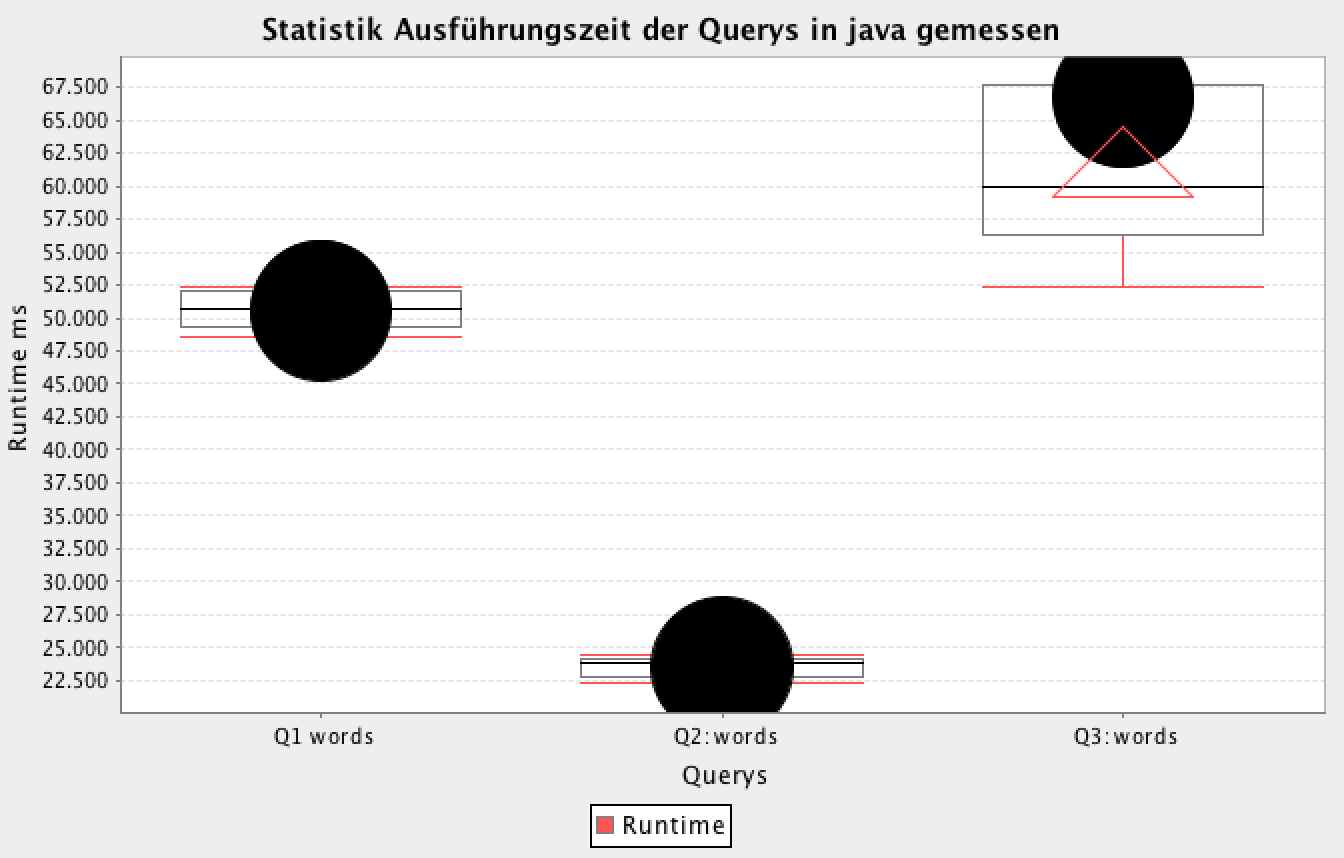
\includegraphics[scale=0.5]{PerformanceHiveInMsWords.png}
\centering
\caption{Performance Hive Querys auf Tabelle Words (unpartitioniert)}
\label{fig:PerfWords}
\end{figure}

\begin{figure}[htb]
\includegraphics[scale=0.5]{PerformanceHiveInMsWordsPartitioned.png}
\centering
\caption{Performance Hive Querys auf Tabelle WordsPartitoned}
\label{fig:PerfWordsPar}
\end{figure}

Die Messungen unterstreichen die bereits gezogenen Schlüsse.

\section{Fazit (Aufgabe 3.3)}

\textbf{Word2Vec}
\begin{itemize}
\item{Scheint grundsätzlich benutzbare Technik für ein Recommender-System zu sein.}
\item{Voraussetzungen: ein themenbezogener Datenbestand als Eingabe (z.B. Amazon Produkt Daten oder Reviews)}
\item{Abbildung von semantischen Relationen: Bewertung anhand einer einzelnen These mit WordNet sehr schwierig.}
\begin{itemize}
\item{Subjektiv liefert Word2Vec aber keine schlechten Resultate.}
\item{Bessere Möglichkeit zur systematischen Bewertung der Ergebnisqualität müsste gefunden werden.}
\end{itemize}
\end{itemize}

\textbf{Hive und Hadoop}
\begin{itemize}
\item{Nicht geeignet, da für einen Recommender zu langsam.}
\begin{itemize}
\item{Datenbestand mit wenigen GB würde auch problemlos in Hauptspeicher passen. Noch wesentlich kleiner im Binärformat.}
\item{Hadoop mit Map-Reduce eigentlich eher für mehrere Terabyte große Daten sinnvoll.}
\end{itemize}
\item{Nicht geeignet, da scheinbar sehr Instabil (zumindest bei uns). Ein Recommender muss mehrere Anfragen gleichzeitig abarbeiten können.}
\item{Nicht geeignet für Clustering, da Mächtigkeit von Map-Reduce sehr eingeschränkt.}
\begin{itemize}
\item{Balancieren von Partitionen vermutlich schlecht umsetzbar.}
\end{itemize}
\end{itemize}

\end{document}
